\section{Background and research questions}
\begin{frame}
	\frametitle{Load and production balancing}
	\begin{columns}
		\begin{column}{0.5\textwidth}
			\begin{itemize}
				\item<1-> The power system frequency measures the power balance.
				\item<2-> It is the responsibility of the TSOs to control the frequency.
				\item<3-> However, it is the power plant owners who can control the frequency.
				\item<4-> The TSOs pay all power plant owners above a certain size to provide frequency control.(droop $\rho =\Delta f/\Delta P$)
			\end{itemize}
		\end{column}
		\begin{column}{0.5\textwidth}
			\begin{figure}
				\includegraphics<1>[width=0.8\textwidth]{./pictures/balance.png}
				\includegraphics<2>[width=0.8\textwidth]{./pictures/balance_statnett.png}
				\includegraphics<3>[width=0.8\textwidth]{./pictures/balance_producers.png}
				\includegraphics<4>[width=0.9\textwidth]{./pictures/speedDroop.tikz}
			\end{figure}
		\end{column}
	\end{columns}
\end{frame}
\begin{frame}
	\frametitle{Hydro power plant}
	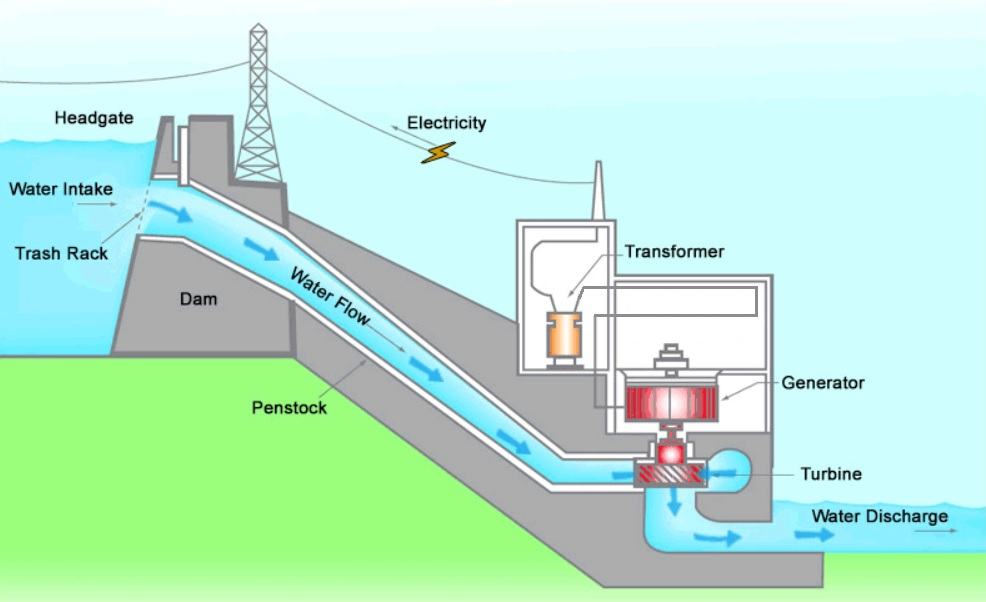
\includegraphics[width=\textwidth]{./pictures/power_plant.png}
\end{frame}
\begin{frame}
	\frametitle{Implementation of the frequency containment process}
	\begin{itemize}
		\item $r(s)$ Reference frequency
		\item $e(s)$ Control error
		\item $f(s)$ Frequency
		\item $c(s)$ Control signal
		\item $g(s)$ Guide vane opening
		\item $\Delta P_m(s)$ Mechanical power
	\end{itemize}
	\includegraphics<1->{./pictures/sys_fcp.tikz}
	\includegraphics<2>{./pictures/fcp_block.tikz}
\end{frame}
\begin{frame}
	\frametitle{The frequency containment process $G_p(s)$ in the power system}	
	\begin{itemize}
		\item $G_J(s)$ represents the swing dynamics of the power plant.
		\item $v_l(s)$ represents stochastic load.
	\end{itemize}
	\includegraphics<1->{./pictures/sys.tikz}
\end{frame}

\begin{frame}
	\frametitle{Stability requirements for frequency control}
	\begin{columns}
			\begin{column}[T]{0.5\textwidth}
			\begin{itemize}
				\item Stability margin from control theory:
				\begin{equation}
					\max |S(j\Omega)| <	M_s
				\end{equation}
			\item where:
				\begin{equation}
						S(s) = \frac{1}{1+G_p(s)G_J(s)}
				\end{equation}
			\end{itemize}
			\includegraphics{./pictures/sys_S.tikz}
		\end{column}
		\begin{column}[T]{0.5\textwidth}
				\includegraphics[width=0.9\textwidth]{./pictures/S_example.tikz}
				%\includegraphics<2>[width=0.8\textwidth]{./pictures/nyquist_L.tikz}
		\end{column}
	\end{columns}
\end{frame}
\begin{frame}
	\frametitle{Performance requirements for frequency control}
	\begin{columns}
			\begin{column}[T]{0.5\textwidth}
			\begin{itemize}
				\item We want to contain frequency deviations.
					\begin{equation}
							\Delta \omega(s) = \frac{G_{J}}{1+G_p(s)G_J(s)}\Delta P_e(s)
					\end{equation}
				\item Define
					\begin{equation}
						G_1(s) = \frac{G_{J}}{1+G_p(s)G_J(s)}
					\end{equation}
			\end{itemize}
		\end{column}
		\begin{column}[T]{0.5\textwidth}
			\includegraphics[width=\textwidth]{./pictures/simulink_bode_compare.tikz}
			\begin{equation}
				|G_1(j\Omega)| < M_p
		\end{equation}
		\end{column}
	\end{columns}
	\includegraphics{./pictures/sys_G1.tikz}
\end{frame}
\begin{frame}
	\frametitle{Future of frequency control}
		\begin{itemize}
			\item Power plants have to show that they fulfill:
				\begin{itemize}
					\item Stability requirement $|S(j\Omega)| < M_s$
					\item Performance requirement $|G_1(j\Omega)| < M_p$
				\end{itemize}
			\item To do this they need models of:
				\begin{itemize}
					\item $G_p(s)$
					\item and $G_J(s)$
				\end{itemize}
		\end{itemize}
	\includegraphics{./pictures/sys.tikz}
\end{frame}
\begin{frame}
	\frametitle{Industry proposed tests}
	\begin{columns}
		\begin{column}{0.3\textwidth}
			\begin{itemize}
				\item Time consuming.
				\item Use system estimate for $G_J(s)$.
				\item Input $r(s)$
				\item Output $\Delta P_e(s)$
			\end{itemize}
		\end{column}
		\begin{column}{0.7\textwidth}
				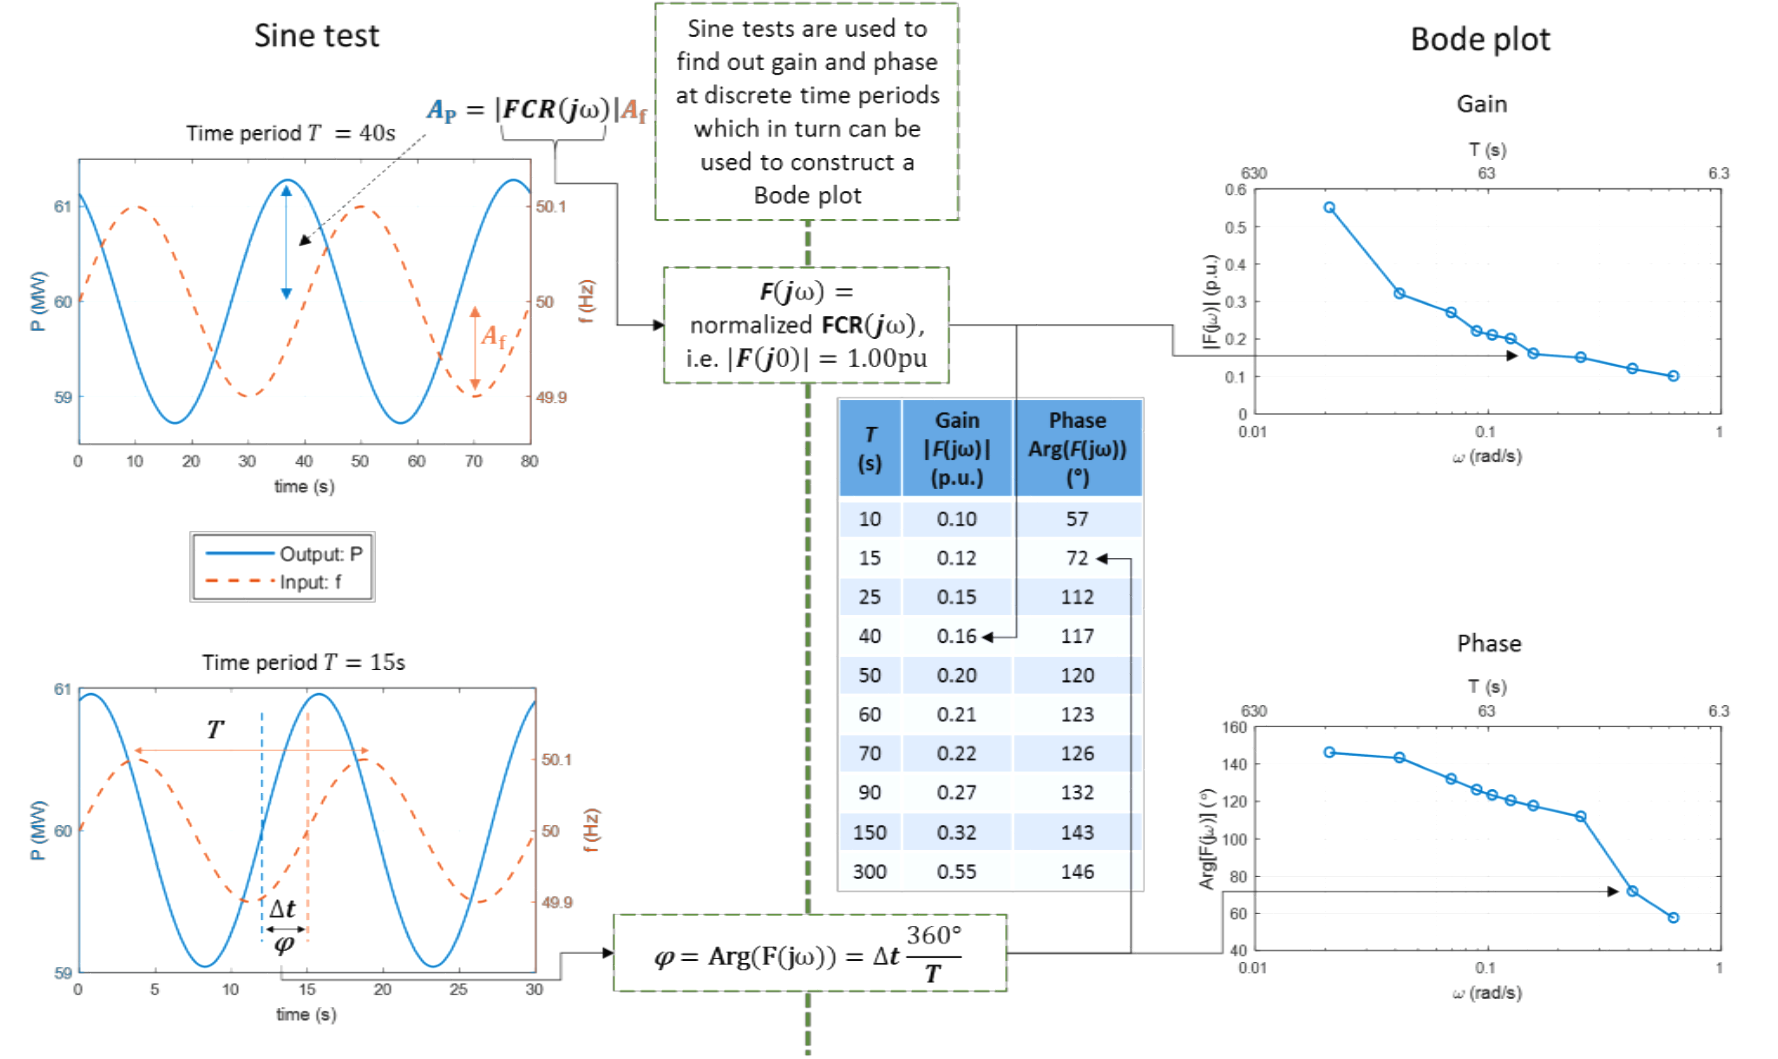
\includegraphics[width=\textwidth]{./pictures/tests.png}
		\end{column}
	\end{columns}
	\includegraphics{./pictures/plant_open.tikz}
\end{frame}
\begin{frame}
	\frametitle{Example from real tests}
	\begin{columns}
		\begin{column}{0.5\textwidth}
			\begin{itemize}
				\item<1-> The power plant needs to be disconnected
				\item<1-> Takes up to 20 hours.
				\item<2-> Only one sine test needed with system identification.
			\end{itemize}
		\end{column}
		\begin{column}{0.5\textwidth}
			\begin{figure}
				\includegraphics<1->[width=\textwidth]{./pictures/aura_signals.tikz}
			\end{figure}
				\includegraphics<1>[width=\textwidth]{./pictures/frd.tikz}
				\includegraphics<2>[width=\textwidth]{./pictures/frd_vs_bj.tikz}
			\end{column}
	\end{columns}
\end{frame}
\begin{frame}
	\frametitle{Motivation}
	\begin{columns}
		\begin{column}{0.5\textwidth}
			\begin{itemize}
				\item<1-> Can we do the tests easier?
				\item<2-> The power system is never really in steady state.
				\item<3-> Can the power plant dynamics be identified from normal operation measurements?
					\end{itemize}
		\end{column}
		\begin{column}{0.5\textwidth}
			\begin{figure}
				\includegraphics<2->[width=\textwidth]{./pictures/aura_pmu.tikz}
			\end{figure}
		\end{column}
	\end{columns}
\end{frame}
\begin{frame}
	\frametitle{Research questions}
	\begin{itemize}
		\item Can power plant dynamics be identified using a PMU?
		\item Can power plant dynamics be identified using control system measurements without disturbing the operation of the plant?  
		\item What is the effect of nonlinearities on the identification?
	\end{itemize}
\end{frame}
